\documentclass[a4paper]{article}
\usepackage{a4wide,amssymb,epsfig,latexsym,multicol,array,hhline,fancyhdr}
\usepackage{matlab-prettifier}
\usepackage{amsmath}
\usepackage{float}
\usepackage{lastpage}
\usepackage[lined,boxed,commentsnumbered]{algorithm2e}
\usepackage{enumerate}
\usepackage{color}
\usepackage{graphicx}
\usepackage{array}
\usepackage{tabularx, caption}
\usepackage{multirow}
\usepackage{multicol}
\usepackage{rotating}
\usepackage{graphics}
\usepackage{geometry}
\usepackage{setspace}
\usepackage{epsfig}
\usepackage{tikz}
\usepackage{url}
\usepackage{listings}
\usepackage{xcolor}
\usepackage{mathptmx}
\usetikzlibrary{arrows,snakes,backgrounds}
\usepackage{hyperref}
\hypersetup{urlcolor=blue,linkcolor=black,citecolor=black,colorlinks=true}

\newtheorem{theorem}{{\bf Theorem}}
\newtheorem{property}{{\bf Property}}
\newtheorem{proposition}{{\bf Proposition}}
\newtheorem{corollary}[proposition]{{\bf Corollary}}
\newtheorem{lemma}[proposition]{{\bf Lemma}}

\AtBeginDocument{\renewcommand*\contentsname{Contents}}
\AtBeginDocument{\renewcommand*\refname{References}}

\definecolor{codegreen}{rgb}{0,0.6,0}
\definecolor{codegray}{rgb}{0.5,0.5,0.5}
\definecolor{codepurple}{rgb}{0.58,0,0.82}
\definecolor{backcolour}{rgb}{0.95,0.95,0.92}

\lstdefinestyle{mystyle}{
    backgroundcolor=\color{backcolour},
    commentstyle=\color{codegreen},
    keywordstyle=\color{magenta},
    numberstyle=\tiny\color{codegray},
    stringstyle=\color{codepurple},
    basicstyle=\ttfamily\footnotesize,
    breakatwhitespace=false,
    breaklines=true,
    captionpos=b,
    keepspaces=true,
    numbers=left,
    numbersep=5pt,
    showspaces=false,
    showstringspaces=false,
    showtabs=false,
    tabsize=2
}
\lstset{style=mystyle}

\setlength{\headheight}{40pt}
\pagestyle{fancy}
\fancyhead{}
\fancyhead[L]{
 \begin{tabular}{rl}
    \begin{picture}(25,15)(0,0)
    \put(0,-8){
\includegraphics[width=8mm, height=8mm]{hcmut.png}}
   \end{picture}&
	\begin{tabular}{l}
		\textbf{\bf \ttfamily University of Technology, Ho Chi Minh City}\\
		\textbf{\bf \ttfamily Faculty of Computer Science and Engineering}
	\end{tabular}
 \end{tabular}
}
\fancyhead[R]{
	\begin{tabular}{l}
		\tiny \bf \\
		\tiny \bf
	\end{tabular}  }
\fancyfoot{}
\fancyfoot[L]{\scriptsize \ttfamily Assignment for Data Engineering - Academic year 2025 - 2026}
\fancyfoot[R]{\scriptsize \ttfamily Page {\thepage}/\pageref{LastPage}}
\renewcommand{\headrulewidth}{0.3pt}
\renewcommand{\footrulewidth}{0.3pt}

\setcounter{secnumdepth}{4}
\setcounter{tocdepth}{3}
\makeatletter
\newcounter {subsubsubsection}[subsubsection]
\renewcommand\thesubsubsubsection{\thesubsubsection .\@alph\c@subsubsubsection}
\newcommand\subsubsubsection{\@startsection{subsubsubsection}{4}{\z@}%
                                     {-3.25ex\@plus -1ex \@minus -.2ex}%
                                     {1.5ex \@plus .2ex}%
                                     {\normalfont\normalsize\bfseries}}
\newcommand*\l@subsubsubsection{\@dottedtocline{3}{10.0em}{4.1em}}
\newcommand*{\subsubsubsectionmark}[1]{}
\makeatother


\begin{document}
\begin{titlepage}
\begin{center}
VIETNAM NATIONAL UNIVERSITY, HO CHI MINH CITY \\
UNIVERSITY OF TECHNOLOGY \\
FACULTY OF COMPUTER SCIENCE AND ENGINEERING
\end{center}

\vspace{1cm}

\begin{figure}[h!]
\begin{center}

\includegraphics[width=3cm]{hcmut.png}
\end{center}
\end{figure}

\vspace{1cm}

\begin{center}
\begin{tabular}{c}
\multicolumn{1}{l}{\textbf{{\Large Data Engineering}}}\\
~~\\
\hline
\\
\textbf{{\Huge Finnhub Streaming Data Pipeline}}\\
\\
\textbf{{\Huge \& Analytics Platform}}\\
\\
\hline
\end{tabular}
\end{center}

\vspace{3cm}

\begin{table}[h]
\begin{tabular}{rrl}
\hspace{5 cm} & Advisor: & Vo Thi Ngoc Chau\\
& Students: & Nguyen Binh Nguyen - 2252545 \\
& & La Quang Huy - 2470736 \\
& & Dang Huynh Minh Tri - 2370007 \\
& & Pham Minh Tri - 2580868 \\
& & To Anh Phat - 2580894 \\
\end{tabular}
\end{table}

\begin{center}
{\footnotesize HO CHI MINH CITY, MAY 2026}
\end{center}
\end{titlepage}

\newpage
\tableofcontents
\newpage

%=============================================================================
\section{Introduction}
%=============================================================================

\subsection{Problem Context}

The cryptocurrency market operates 24 hours a day, seven days a week, generating
a continuous stream of high-frequency trade data across dozens of exchanges.
Analysts and investors face two distinct but related challenges.

On the real-time side, traders need to detect price movements, volume spikes,
and order-flow anomalies within seconds. Traditional relational databases cannot
ingest or serve this data volume at the required latency.

On the analytical side, understanding long-term trends, volatility cycles,
seasonal patterns, and risk-adjusted returns demands clean, consistent historical
data in a format built for large-scale OLAP queries rather than row-level
lookups.

Off-the-shelf solutions either address one of these needs or come with
significant vendor lock-in and cost. The project therefore targets an
open-source, self-hosted system that unifies both workloads within a single
reproducible infrastructure.

\subsection{Solution}

An end-to-end data engineering pipeline that ingests, processes, stores, and
visualises real-time cryptocurrency trade data, while also storing historical
data in a data warehouse for business intelligence and analysis.

\begin{figure}[H]
\centering
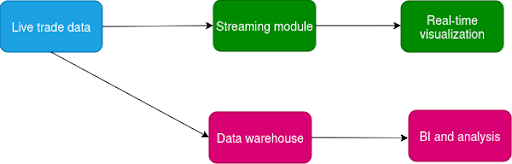
\includegraphics[width=0.8\textwidth]{solution.png}
\caption{Solution overview}
\end{figure}

This report covers the design and implementation of such a platform using modern
open-source big data technologies. The system ingests live cryptocurrency trade
data from the Finnhub WebSocket API, routes it through a streaming layer into a
distributed NoSQL database for operational queries, and in parallel runs a
multi-layered data warehouse for long-term analytical workloads.

The \textbf{streaming pipeline} captures tick-level trade events from Finnhub
in real time, publishes them to Apache Kafka, processes them with PySpark
Structured Streaming, and writes raw trades, 1-minute OHLCV aggregations, and
the latest price per symbol into Apache Cassandra. Grafana reads from Cassandra
to render live dashboards.

The \textbf{batch pipeline} applies a \emph{medallion architecture}
(Bronze $\rightarrow$ Silver $\rightarrow$ Gold) to historical cryptocurrency CSV
datasets using PySpark and Delta Lake on MinIO object storage. The Gold layer
produces a Kimball-style star schema that Trino exposes as SQL and Superset
visualises for long-term analytics.

The entire infrastructure runs in Docker Compose, so the full stack (Zookeeper,
Kafka, Cassandra, MinIO, Hive Metastore, Trino, Grafana, and Superset) starts
on a single machine with one command. The system tracks three assets:
\textbf{Bitcoin (BTC)}, \textbf{Ethereum (ETH)}, and \textbf{Litecoin (LTC)},
covering daily OHLCV records from January 2018 to July 2024, totalling 7,045
validated records after cleaning.

%=============================================================================
\section{System Architecture}
%=============================================================================

\subsection{High-Level Overview}

The architecture consists of five logical layers:

\begin{enumerate}
    \item \textbf{Ingestion:} Finnhub WebSocket API $\rightarrow$ FinnhubProducer $\rightarrow$ Kafka
    \item \textbf{Stream Processing:} Kafka $\rightarrow$ Spark Structured Streaming $\rightarrow$ Cassandra
    \item \textbf{Operational Visualization:} Cassandra $\rightarrow$ Grafana
    \item \textbf{Batch / Warehouse:} CSV datasets $\rightarrow$ PySpark notebooks $\rightarrow$ Delta Lake on MinIO
    \item \textbf{Analytical Visualization:} MinIO (Delta) $\rightarrow$ Trino $\rightarrow$ Superset
\end{enumerate}

\begin{figure}[H]
\centering
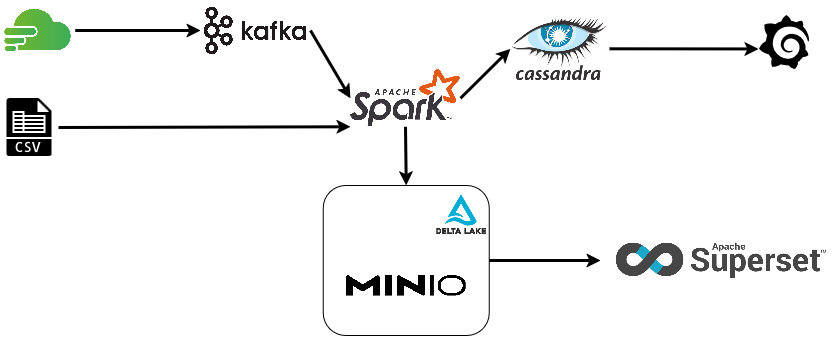
\includegraphics[width=0.85\textwidth]{architecture.png}
\caption{High-level system architecture}
\end{figure}

\subsection{Technology Stack}

\subsubsection{Streaming Layer}

\begin{table}[H]
\centering
\begin{tabular}{|l|l|}
\hline
\textbf{Component} & \textbf{Role} \\
\hline
Apache Kafka 7.6.0 (Confluent) & Distributed message broker; topic \texttt{finnhub-trades} \\
\hline
Apache Zookeeper 3.8 & Kafka cluster coordination \\
\hline
PySpark 4.0 / Spark Structured Streaming & Stateful stream processor \\
\hline
Apache Cassandra 4.1 & Low-latency NoSQL store for operational queries \\
\hline
Grafana 12 & Live dashboard connected to Cassandra \\
\hline
\end{tabular}
\caption{Streaming layer components}
\end{table}

\subsubsection{Batch / Warehouse Layer}

\begin{table}[H]
\centering
\begin{tabular}{|l|l|}
\hline
\textbf{Component} & \textbf{Role} \\
\hline
PySpark 4.0 + Delta Lake 4.0 & ETL notebooks (Bronze / Silver / Gold) \\
\hline
MinIO & S3-compatible object storage hosting Delta tables \\
\hline
Apache Hive Metastore 4.0 & Table registry for Trino's Delta connector \\
\hline
Trino 468 & Distributed SQL query engine with Delta Lake catalog \\
\hline
Apache Superset 4.0 & Self-serve BI and dashboard platform \\
\hline
\end{tabular}
\caption{Batch / warehouse layer components}
\end{table}

All 11 services run on a shared \texttt{streaming-network} Docker bridge.
Kafka UI (port 8080) and MinIO Console (port 9011) provide web UIs for topic
inspection and bucket browsing respectively.

%=============================================================================
\section{Streaming Data Pipeline}
%=============================================================================

\subsection{FinnhubProducer}

The producer (\texttt{FinnhubProducer/src/producer.py}) connects to the Finnhub
WebSocket endpoint, subscribes to trade events for the configured symbols, and
forwards each event as a JSON message to the Kafka topic \texttt{finnhub-trades}.

\textbf{Event schema published to Kafka:}
\begin{lstlisting}[language=Python]
{
    "symbol":     "AAPL",        # ticker symbol
    "price":      189.42,        # trade price
    "volume":     120.0,         # trade volume
    "timestamp":  1718000000000, # Unix milliseconds
    "conditions": ["1"]          # trade condition codes
}
\end{lstlisting}

To handle Kafka broker startup latency, the producer retries the connection with
exponential backoff (10 attempts, 5-second delay).

\subsection{Stream Processor}

The stream processor (\texttt{StreamProcessor/src/processor.py}) is a PySpark
Structured Streaming job that reads from Kafka and runs \textbf{three parallel
write streams} against Cassandra.

\subsubsection{Query 1: Raw Trades}
This query writes every parsed trade event into \texttt{trading.trades} using
\texttt{foreachBatch}, with no aggregation, preserving a full tick-level audit trail.

\subsubsection{Query 2: 1-Minute OHLCV Aggregations}
This query groups trades into 1-minute tumbling windows with a 1-minute watermark,
computing open, high, low, close, total volume, and trade count. Spark flushes
the results to \texttt{trading.trades\_agg\_1m} every 5 seconds.

\begin{lstlisting}[language=Python]
agg_df = (
    parsed_df
    .withWatermark("trade_time", "1 minute")
    .groupBy("symbol", "trade_date",
             F.window("trade_time", "1 minute").alias("w"))
    .agg(
        F.min_by("price", "trade_time").alias("open_price"),
        F.max_by("price", "trade_time").alias("close_price"),
        F.max("price").alias("high_price"),
        F.min("price").alias("low_price"),
        F.sum("volume").alias("total_volume"),
    )
)
\end{lstlisting}

\subsubsection{Query 3: Latest Price per Symbol}
For each micro-batch, the query selects the most recent trade per symbol by
\texttt{trade\_time} and upserts it into \texttt{trading.latest\_price}. Because
the Cassandra primary key is \texttt{symbol} alone, each write overwrites the
previous record, keeping an always-current ticker for the dashboard.

\subsection{Cassandra Schema}

The keyspace \texttt{trading} contains three tables, each partition-keyed to
match the most common query patterns.

\begin{table}[H]
\centering
\begin{tabular}{|l|l|l|}
\hline
\textbf{Table} & \textbf{Partition Key} & \textbf{Clustering Key} \\
\hline
\texttt{trades} & \texttt{(symbol, trade\_date)} & \texttt{trade\_time DESC} \\
\hline
\texttt{trades\_agg\_1m} & \texttt{(symbol, trade\_date)} & \texttt{window\_start DESC} \\
\hline
\texttt{latest\_price} & \texttt{symbol} & none \\
\hline
\end{tabular}
\caption{Cassandra table partition design}
\end{table}

Partitioning by \texttt{(symbol, trade\_date)} bounds each partition to one day
of trades per symbol, preventing hot partitions during high-volume sessions. The
\texttt{DESC} clustering order means Cassandra returns the most recent rows
first, cutting dashboard query latency.

\subsection{Grafana Live Dashboard}

\begin{figure}[H]
\centering
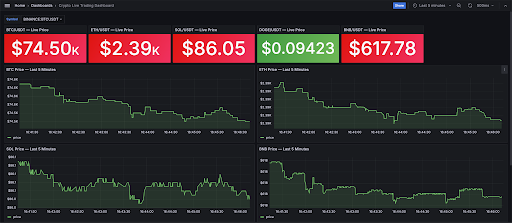
\includegraphics[width=\textwidth]{stream-dashboard.png}
\caption{Grafana live trading dashboard reading from Cassandra in real time}
\end{figure}

The Grafana dashboard provides an at-a-glance view of the streaming pipeline's
output. The top row displays five large-format stat panels, each showing the
latest traded price for a symbol: BTC/USDT at \$74.50k, ETH/USDT at \$2.39k,
SOL/USDT at \$86.05, DOGE/USDT at \$0.09423, and BNB/USDT at \$617.78. These
values come directly from the \texttt{trading.latest\_price} Cassandra table,
which Query 3 of the stream processor overwrites with each new micro-batch.

Below the stat panels, four time-series charts plot the price of BTC, ETH,
SOL, and another asset over a rolling 5-minute window, with sub-minute
granularity. The data feeds from \texttt{trading.trades\_agg\_1m} via the
Grafana Cassandra data-source plugin. Together the two layers of the dashboard
serve different operational needs: the stat panels give traders an immediate
price check, while the line charts expose short-term momentum and micro-volatility
that a single number cannot capture.

%=============================================================================
\section{Batch Data Pipeline: Medallion Architecture}
%=============================================================================

The batch pipeline processes historical price data for BTC, ETH, and LTC
through three notebook stages stored in \texttt{BatchProcessor/notebooks/}.
Each stage writes Delta Lake tables to MinIO at
\texttt{s3a://crypto-warehouse/\{layer\}/}.

\subsection{Bronze Layer}

Notebook \texttt{01\_bronze\_layer.ipynb} reads the raw CSV files
(\texttt{BITCOIN24.csv}, \texttt{ETHEREUM.csv}, \texttt{LITECOIN24.csv}) and
appends them to a single Delta table at
\texttt{s3a://crypto-warehouse/bronze/} with minimal transformation. The
notebook enriches each row with three metadata columns (\texttt{asset\_symbol},
\texttt{source\_file}, \texttt{ingestion\_ts}) and treats the result as the
immutable raw record of all source data.

\begin{table}[H]
\centering
\begin{tabular}{|l|c|}
\hline
\textbf{Asset} & \textbf{Rows Ingested} \\
\hline
BTC & 2,250 \\
\hline
ETH & 2,404 \\
\hline
LTC & 2,404 \\
\hline
\textbf{Total} & \textbf{7,058} \\
\hline
\end{tabular}
\caption{Bronze layer row counts per asset}
\end{table}

\subsection{Silver Layer}

Notebook \texttt{02\_silver\_layer.ipynb} reads from the Bronze table, applies
validation and type casting, then derives two computed columns:
\texttt{daily\_return} $= (\text{close} - \text{open}) / \text{open}$ and
\texttt{price\_range} $= \text{high} - \text{low}$.

Any row that contains a NULL or non-positive OHLCV field, or whose
\texttt{trade\_date} cannot parse as either \texttt{dd-MM-yyyy} or
\texttt{yyyy-MM-dd}, goes to a separate \texttt{silver/ohlcv\_rejected} Delta
table rather than the main Silver table. Of the 7,058 Bronze rows, 13 fail
validation (0.18\%), all due to missing volume and market cap values in certain
source CSV files.

\subsection{Gold Layer: Star Schema}

Notebook \texttt{03\_gold\_layer.ipynb} transforms the cleaned Silver data into
a \textbf{Kimball-style star schema} optimised for OLAP queries, writing four
Delta tables to \texttt{s3a://crypto-warehouse/gold/}.

\subsubsection{Fact Table: fact\_daily\_ohlc}

\begin{table}[H]
\centering
\begin{tabular}{|l|l|l|}
\hline
\textbf{Column} & \textbf{Type} & \textbf{Description} \\
\hline
trade\_key & INT & Surrogate primary key \\
\hline
asset\_key & INT & FK $\rightarrow$ dim\_asset \\
\hline
date\_key & INT & FK $\rightarrow$ dim\_date (YYYYMMDD) \\
\hline
open\_price & DOUBLE & Opening price \\
\hline
high\_price & DOUBLE & Daily high \\
\hline
low\_price & DOUBLE & Daily low \\
\hline
close\_price & DOUBLE & Closing price \\
\hline
volume & LONG & Trading volume \\
\hline
market\_cap & DOUBLE & Market capitalisation \\
\hline
daily\_return & DOUBLE & (close $-$ open) / open \\
\hline
price\_range & DOUBLE & high $-$ low \\
\hline
loaded\_timestamp & STRING & Source ingestion timestamp \\
\hline
data\_source & STRING & Source CSV file name \\
\hline
\end{tabular}
\caption{fact\_daily\_ohlc schema (7,045 rows)}
\end{table}

\subsubsection{Dimension Tables}

\textbf{dim\_asset} (3 rows):
\begin{table}[H]
\centering
\begin{tabular}{|l|l|l|}
\hline
\textbf{Column} & \textbf{Type} & \textbf{Description} \\
\hline
asset\_key & INT & Surrogate PK \\
\hline
asset\_symbol & STRING & BTC / ETH / LTC \\
\hline
asset\_name & STRING & Bitcoin / Ethereum / Litecoin \\
\hline
asset\_category & STRING & Layer1 \\
\hline
exchange & STRING & Spot \\
\hline
is\_active & BOOLEAN & Active flag \\
\hline
\end{tabular}
\caption{dim\_asset schema}
\end{table}

\textbf{dim\_date} (2,403 rows, full date spine from 2018-01-01 to 2024-07-31):
\begin{table}[H]
\centering
\begin{tabular}{|l|l|}
\hline
\textbf{Column} & \textbf{Description} \\
\hline
date\_key & Integer PK (YYYYMMDD) \\
\hline
full\_date & DATE \\
\hline
year, quarter, month & Calendar decomposition \\
\hline
month\_name, day\_name & Human-readable labels \\
\hline
week\_of\_year, day\_of\_week & ISO week/day numbers \\
\hline
is\_weekend & BOOLEAN; flags weekends for seasonality analysis \\
\hline
\end{tabular}
\caption{dim\_date schema}
\end{table}

\textbf{dim\_time} (86,400 rows, one row per second of the day):
Provides \texttt{hour}, \texttt{minute}, \texttt{second}, and \texttt{am\_pm}
for sub-daily analysis of streaming data.

%=============================================================================
\section{Analytical Layer: Trino and Superset}
%=============================================================================

\subsection{Trino Configuration}

Trino connects to the Gold Delta tables through the \textbf{Delta Lake
connector}, using Hive Metastore (HMS) as the table registry and MinIO as the
underlying file storage.

\begin{lstlisting}[language=bash]
# trino/etc/catalog/delta.properties
connector.name=delta_lake
hive.metastore.uri=thrift://hive-metastore:9083
fs.native-s3.enabled=true
s3.endpoint=http://minio:9000
s3.aws-access-key=minioadmin
s3.aws-secret-key=minioadmin123
s3.path-style-access=true
delta.register-table-procedure.enabled=true
\end{lstlisting}

The Gold tables need registering only once via the \texttt{register\_table}
system procedure; the HMS Derby volume preserves the metadata across restarts:

\begin{lstlisting}[language=SQL]
CREATE SCHEMA IF NOT EXISTS delta.gold
    WITH (location = 's3a://crypto-warehouse/gold/');

CALL delta.system.register_table(
    schema_name => 'gold',
    table_name  => 'fact_daily_ohlc',
    table_location => 's3a://crypto-warehouse/gold/fact_daily_ohlc'
);
\end{lstlisting}

\subsection{Superset Dashboards}

Two dashboards are created via the Superset REST API using Python automation
scripts (\texttt{scripts/create\_superset\_dashboard.py} and
\texttt{scripts/create\_longterm\_dashboard.py}).

\subsubsection{Dashboard 1: Crypto Analytics (Operational View)}

\begin{table}[H]
\centering
\begin{tabular}{|l|l|p{7cm}|}
\hline
\textbf{Chart} & \textbf{Type} & \textbf{Description} \\
\hline
Close Price Over Time & Line & Daily closing price for BTC / ETH / LTC \\
\hline
Daily Return Over Time & Line & Average daily return (\%) per asset \\
\hline
Volume Over Time & Bar & Monthly total trading volume per asset \\
\hline
Price Range (High$-$Low) & Line & Weekly average intraday spread \\
\hline
Asset Summary Table & Table & Max / min / avg close, avg daily return, total volume \\
\hline
\end{tabular}
\caption{Dashboard 1: Crypto Analytics charts}
\end{table}

\subsubsection{Dashboard 2: Crypto Long-Term Analytics (Warehouse View)}

\begin{table}[H]
\centering
\begin{tabular}{|l|l|p{7cm}|}
\hline
\textbf{Chart} & \textbf{Type} & \textbf{Description} \\
\hline
Normalized Performance & Line & Base-100 indexed from 2018-01-01; shows relative growth \\
\hline
Annual Return \% & Bar & Year-over-year price return per asset \\
\hline
Annualized Volatility & Bar & Std dev of daily returns $\times \sqrt{252}$ per year \\
\hline
Monthly Seasonality & Bar & Average daily return by calendar month \\
\hline
Weekend vs Weekday & Bar & Average return on weekends vs weekdays (uses \texttt{dim\_date.is\_weekend}) \\
\hline
Market Cap Share & Pie & Average market cap distribution across BTC, ETH, LTC \\
\hline
Quarterly High/Avg/Low & Table & OHLCV aggregated at quarter level per asset \\
\hline
\end{tabular}
\caption{Dashboard 2: Long-Term Analytics charts}
\end{table}

Each Dashboard 2 chart runs against a \textbf{virtual dataset}, a SQL view
defined inside Superset that joins \texttt{fact\_daily\_ohlc} with
\texttt{dim\_asset} and \texttt{dim\_date} to surface human-readable columns
such as \texttt{asset\_symbol}, \texttt{year}, \texttt{month}, and
\texttt{is\_weekend}. Trino executes the join at query time directly against
the Delta tables in MinIO, so no data duplication occurs.

\subsubsection{Dashboard 2: Analysis Results}

\textbf{Normalized Performance (Base 100, Jan 2018)}

\begin{figure}[H]
\centering
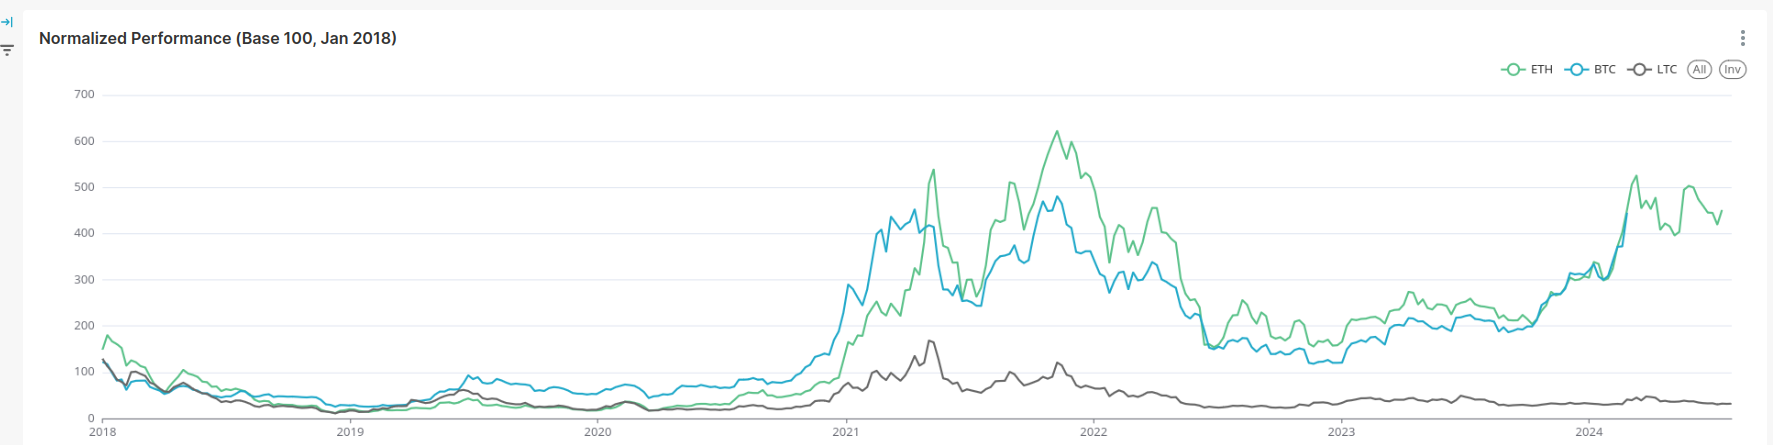
\includegraphics[width=\textwidth]{normalized_performance.png}
\caption{Normalized price performance, base 100 from January 2018}
\end{figure}

The chart re-bases all three assets to 100 at the start of 2018 so that
growth rates are comparable regardless of absolute price differences. BTC and
ETH both collapsed through 2018 and remained below the baseline until 2020.
The 2021 bull run pushed ETH to a peak of roughly 630 and BTC to around 420,
with ETH outperforming on a relative basis during that cycle. After the 2022
crash both assets fell back toward 100, then recovered strongly through
2023-2024 to approximately 430-500 by mid-2024. LTC told a very different
story: its index never meaningfully recovered above 100 after the 2018 crash
and by 2024 sits around 20-30, representing a real loss of roughly 70-80\%
relative to the January 2018 entry point.

\textbf{Annual Return \% by Year}

\begin{figure}[H]
\centering
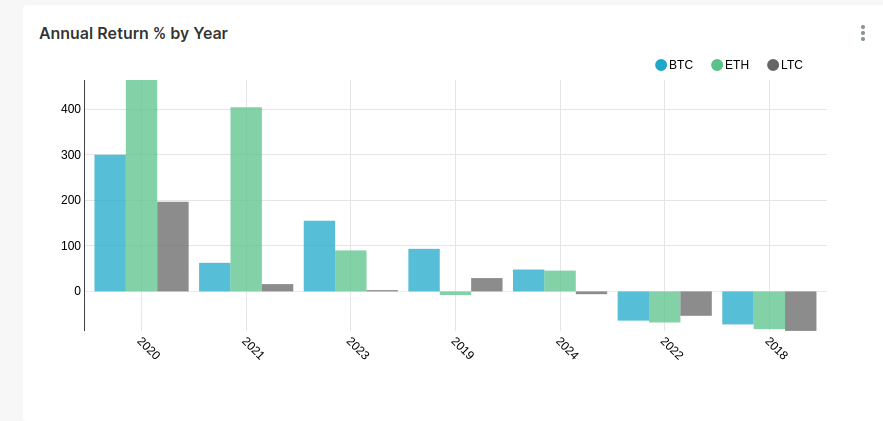
\includegraphics[width=0.85\textwidth]{annual_return.png}
\caption{Year-over-year price return per asset (\%)}
\end{figure}

The bar chart shows the full-year price return for each asset since 2018.
2020 and 2021 stand out as the two strongest bull years: ETH gained
approximately 450\% in 2020 and 400\% in 2021, while BTC returned 300\% and
60\% respectively. By contrast, 2018 and 2022 were deep bear years with
double-digit negative returns across all three assets. BTC led the recovery
in 2023 with a roughly 150\% return, while ETH followed at around 90\% and
LTC turned slightly negative. The chart reinforces that cryptocurrency annual
returns are highly binary: years are either strongly positive or strongly
negative, with very little middle ground.

\textbf{Annualized Volatility by Year}

\begin{figure}[H]
\centering
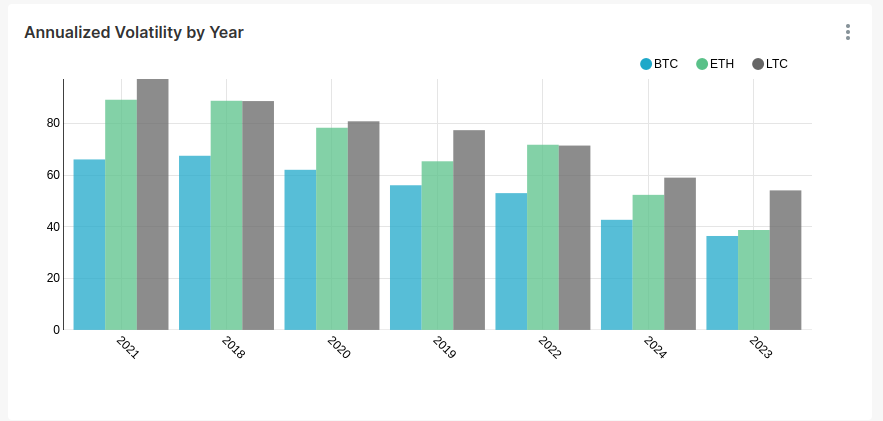
\includegraphics[width=0.85\textwidth]{annualized_volatility.png}
\caption{Annualized volatility (\%) computed as $\sigma_{\text{daily}} \times \sqrt{252}$}
\end{figure}

Even in the calmest year on record (2023), all three assets registered
annualized volatility above 35\%, which is two to three times the typical
level for equity indices. Peak volatility occurred in 2021 for all assets,
with LTC reaching around 95\% and ETH around 88\%. 2018, another year of
extreme price movement, also showed elevated volatility near 87-90\% for ETH
and LTC. BTC consistently shows the lowest volatility among the three,
reflecting its larger market capitalization and deeper liquidity. The data
confirms that crypto volatility does not simply spike in bear years: the 2021
bull run was equally turbulent.

\textbf{Monthly Seasonality (Avg Daily Return \%)}

\begin{figure}[H]
\centering
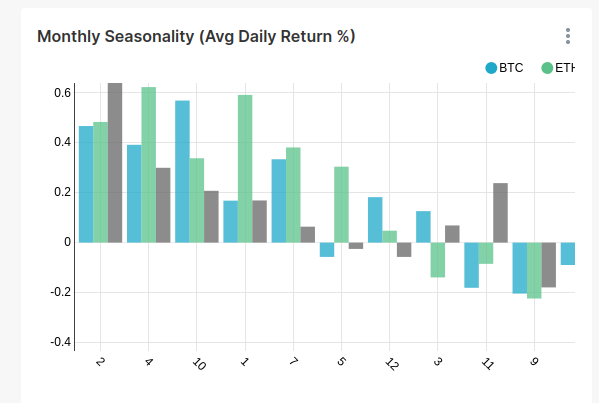
\includegraphics[width=0.85\textwidth]{monthly_seasonality.png}
\caption{Average daily return by calendar month, aggregated across 2018-2024}
\end{figure}

Aggregating six years of daily returns by calendar month reveals a consistent
seasonal pattern. February (month 2) and April (month 4) produce the highest
average daily returns for both BTC and ETH, at roughly 0.46-0.63\% per day.
October (month 10) also shows positive seasonality. September (month 9) and
November (month 11) are the weakest months, with average daily returns turning
negative. This pattern partially mirrors the equity market's well-known
``Sell in May'' effect but with different peak and trough months, likely
driven by the distinct investor base and halving cycle dynamics of the crypto
market.

\textbf{Average Market Cap Share by Asset}

\begin{figure}[H]
\centering
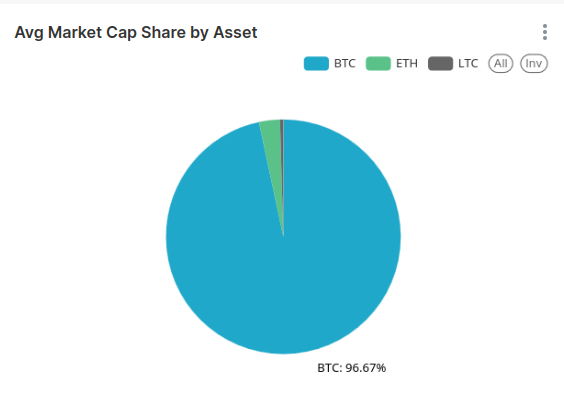
\includegraphics[width=0.7\textwidth]{market_cap_share.png}
\caption{Average market capitalisation share across the 2018-2024 period}
\end{figure}

Across the full 2018-2024 dataset, BTC accounts for 96.67\% of the combined
average market capitalisation of the three tracked assets. ETH holds a small
but visible slice at roughly 3\%, while LTC's share is negligible. This
dataset covers only three assets, so the chart does not represent the full
crypto market, but it illustrates BTC's outsized dominance even within a
comparison that includes Ethereum. The result is consistent with the
normalised performance chart: BTC's absolute price and circulating supply both
far exceed LTC's, compounding its market cap lead throughout the period.

%=============================================================================
\section{Key Technical Highlights}
%=============================================================================

\subsection{Delta Lake on MinIO}

Delta Lake provides ACID transactions and time-travel over Parquet files stored
in MinIO. Each layer's Delta log (\texttt{\_delta\_log/}) records every write
operation, giving full lineage tracing from raw CSV to the Gold star schema.
The Gold layer enables Delta column mapping
(\texttt{delta.columnMapping.mode=name}) to handle column names with spaces
inherited from source CSVs.

\subsection{Spark Structured Streaming: Watermarks and Late Data}

Query 2 applies a \textbf{1-minute watermark} on \texttt{trade\_time}, telling
Spark to hold state for each 1-minute window for one extra minute after the
window closes. This absorbs network jitter and late-arriving events before
Spark finalises the OHLCV aggregate and commits it to Cassandra.

\subsection{Cassandra Partition Design}

The composite partition key \texttt{(symbol, trade\_date)} caps each partition
at one day of trades per symbol, preventing unbounded growth. It also aligns
with the most common dashboard query pattern (all trades for a given symbol on
a given day), which becomes a single-partition read rather than a
scatter-gather. The \texttt{latest\_price} table uses \texttt{symbol} alone as
its primary key, turning every Spark upsert into an idempotent single-row
overwrite.

\subsection{End-to-End Container Isolation}

All 11 services share the \texttt{streaming-network} Docker bridge. Container
names carry the \texttt{finnhub-} prefix to avoid conflicts with other Compose
projects on the same host. Port mappings are assigned to avoid collisions:

\begin{table}[H]
\centering
\begin{tabular}{|l|l|l|}
\hline
\textbf{Service} & \textbf{Host Port} & \textbf{Container Port} \\
\hline
Kafka & 9092 & 9092 \\
\hline
Cassandra & 9042 & 9042 \\
\hline
Kafka UI & 8080 & 8080 \\
\hline
Grafana & 3000 & 3000 \\
\hline
MinIO S3 API & 9010 & 9000 \\
\hline
MinIO Console & 9011 & 9001 \\
\hline
Hive Metastore & 9083 & 9083 \\
\hline
Trino & 8081 & 8080 \\
\hline
Superset & 8088 & 8088 \\
\hline
\end{tabular}
\caption{Host-to-container port mappings}
\end{table}

%=============================================================================
\section{Data Flow Summary}
%=============================================================================

\begin{enumerate}
    \item \textbf{Finnhub WebSocket} pushes tick-level trade events for BTC,
    ETH, and LTC symbols.
    \item \textbf{FinnhubProducer} serialises each trade to JSON and publishes
    it to Kafka topic \texttt{finnhub-trades}.
    \item \textbf{StreamProcessor} (PySpark) reads from Kafka, parses the JSON
    payload, and runs three concurrent write streams to Cassandra: raw trades
    into \texttt{trading.trades}, 1-minute OHLCV aggregations into
    \texttt{trading.trades\_agg\_1m}, and the latest price per symbol into
    \texttt{trading.latest\_price}.
    \item \textbf{Grafana} reads from Cassandra and renders live price and
    volume dashboards.
    \item \textbf{Batch notebooks} process historical CSV data through the
    Bronze $\rightarrow$ Silver $\rightarrow$ Gold pipeline, writing Delta Lake
    tables to MinIO at each stage.
    \item \textbf{Trino} exposes the Gold Delta tables through the Delta Lake
    catalog, with HMS supplying table metadata.
    \item \textbf{Superset} queries Trino and renders two analytical dashboards
    covering the operational view and long-term analytics.
\end{enumerate}

%=============================================================================
\section{Conclusion}
%=============================================================================

This project builds a complete, production-grade data engineering pipeline that
spans real-time streaming and long-term analytical workloads.

On the streaming side, PySpark ingests trade events from Finnhub through Kafka
into Cassandra in sub-second latency, computing 1-minute OHLCV candles with
watermark-based late-data handling. On the warehouse side, a three-layer
medallion architecture enforces data quality at each stage, and the Gold star
schema supports efficient OLAP queries without data duplication.

Trino pushes query execution directly to the Delta Parquet files in MinIO,
avoiding unnecessary data movement. Superset virtual datasets join fact and
dimension tables at query time, delivering flexible analytics without
materialised views.

The entire 11-service stack lives in a single \texttt{docker-compose.yml},
so \texttt{docker compose up --build} fully reproduces the environment on any
machine.

\begin{table}[H]
\centering
\begin{tabular}{|l|c|}
\hline
\textbf{Component} & \textbf{Count / Size} \\
\hline
Docker services & 11 \\
\hline
Kafka topics & 1 (\texttt{finnhub-trades}) \\
\hline
Cassandra tables & 3 \\
\hline
Delta Lake layers & 3 (Bronze / Silver / Gold) \\
\hline
Gold dimension tables & 3 (dim\_asset, dim\_date, dim\_time) \\
\hline
Gold fact table rows & 7,045 \\
\hline
Trino catalogs & 1 (delta) \\
\hline
Superset dashboards & 2 \\
\hline
Superset charts & 12 \\
\hline
Total pipeline stages & 7 \\
\hline
\end{tabular}
\caption{Project statistics summary}
\end{table}

\end{document}
